\documentclass[runningheads]{llncs}

\usepackage{iftex}
\ifPDFTeX
  \PackageError{short}{This manuscript must be built with XeLaTeX}{}
\else
  \usepackage{fontspec}
\fi
\usepackage{amsmath,amssymb}
\usepackage{booktabs}
\usepackage{graphicx}
\usepackage{xcolor}
\usepackage{hyperref}
\usepackage{algorithm}
\usepackage{algpseudocode}
\renewcommand\UrlFont{\color{blue}\rmfamily}
\urlstyle{rm}
\graphicspath{{figures/}}
\emergencystretch=1.5em

\begin{document}

% ISDS 2026 submission category: long paper (12--15 pages, references included).
\title{Stress-Testing Product-Gated Clustering and Bounded Priority Ranking
for Flood-Rescue Reports: A Synthetic Study}
\titlerunning{Stress-Testing Flood-Rescue Report Clustering and Ranking}

\author{Thanh-Trong Nguyen\inst{1}\orcidID{0009-0007-6976-5131}\thanks{Corresponding author.} \and
Ngoc-Anh Le\inst{1}\orcidID{0009-0006-7453-1009} \and
Nhu-Quynh Nguyen\inst{1}\orcidID{0009-0008-7396-697X} \and
Tuong-Hung Cao\inst{1}\orcidID{0009-0003-5886-2666} \and
Hung-Thinh Ngo\inst{1}\orcidID{0009-0004-8668-4462} \and
Thanh-Khoa Nguyen\inst{1}\orcidID{0000-0002-0012-1158}}
\authorrunning{T.-T. Nguyen et al.}
\institute{College of Information and Communication Technology,
Can Tho University, Can Tho, Vietnam\\
\email{ngthtrong204@gmail.com}}

\maketitle

\begin{abstract}
Operational flood streams contain duplicate, incomplete, and adversarial
reports, while clustering and priority scores are often evaluated without
measuring their scheduling consequences. We audit a fail-closed batch
pipeline in which observable reports form a sparse graph, unresolved reports
go to review, duplicate families feed a bounded score, and evaluator-only
truth is joined after predicted-cluster scheduling. The clustering benchmark
contains 80 synthetic runs from generator 3.0.0: additive Louvain has mean
ARI $0.9191$, product Leiden $0.9165$, and product Louvain $0.9072$.
Product minus independently tuned additive is $-0.0118$ (bootstrap 95\% CI
$[-0.0226,-0.0024]$), but its Holm-adjusted test is not significant
($p=.2560$). A matched-density comparison reverses the point estimate but is
also inconclusive. In a separate candidate-4.1 bundle, the revised score has
NDCG@5 $0.6669$ versus $0.6763$ for a random comparator and does not show a
general alignment advantage; exact duplicates are invariant but coordinated
high-confidence campaigns remain a failure mode. Dispatch results similarly
show no general benefit over the legacy score and a clear cost relative to
nearest-first. These are synthetic, within-generator diagnostics:
boundedness and clustering accuracy do not establish source authenticity,
policy validity, field benefit, or deployment readiness.
\keywords{Flood rescue \and Graph clustering \and Synthetic stress test \and
Priority ranking \and Negative results.}
\end{abstract}

\section{Introduction and Related Work}

During emergencies, crisis streams mix repeated reports of one event with
nearby but distinct events, missing fields, and nonincident noise. Social-sensor
and emergency-message research addresses volume, verification, and event
extraction~\cite{sakaki2010earthquake}. CrisisMMD and FloodNet capture useful
disaster modalities, although FloodNet is an aerial post-flood
scene-understanding dataset rather than a multimodal report stream
\cite{alam2018crisismmd,rahnemoonfar2021floodnet}. These resources do not
jointly provide physical-incident linkage, rescue priority, and field dispatch
outcomes.

\paragraph{Social sensing and event extraction.}
Social-media users can act as real-time sensors~\cite{sakaki2010earthquake},
but the usual endpoint is event detection or classification rather than the
consequences of sending a field resource to a predicted incident.

\paragraph{Consolidation and clustering.}
Graph community detection with Louvain or Leiden
\cite{blondel2008louvain,traag2019leiden}, and density methods such as DBSCAN
and HDBSCAN~\cite{ester1996dbscan} offer plausible consolidation mechanisms.
Multiplicative spatial--range terms occur in bilateral filtering
\cite{tomasi1998bilateral}; we adapt that structure to a product graph, while
testing the exact gate and its bounds here.

\paragraph{Humanitarian logistics and dispatch.}
Relief-routing models expose competing equity, efficacy, and efficiency
objectives~\cite{gralla2014review}. We use this perspective to motivate a
bounded priority ranking, but boundedness is not an expert-endorsed rescue
policy. A key gap is propagation of false splits, merges, and noise into a
scheduler that cannot consult incident truth.

We address these gaps with a fail-closed batch pipeline: reports with
observable location and time enter a sparse graph, incomplete reports go to
manual review, duplicate families feed a bounded ranking, and evaluator-only
truth joins after predicted-cluster scheduling. We ask: (RQ1) does
independently selected product composition improve clustering over additive
composition? (RQ2) does the duplicate-aware score align with an independently
generated benefit under report-level stress tests? (RQ3) how do predicted
split, merge, and noise errors propagate into dispatch? The questions use two
explicitly separated artifact bundles.

The contributions are (i) an observable-only pipeline with explicit review and
evaluator boundaries; (ii) auditable threshold statements and a proposed
duplicate-aware score; and (iii) a paired diagnostic reporting clustering,
ranking, dispatch, and adverse results. We emphasize that the primary
scientific value of this study lies not in a performance improvement but in
the auditable negative and boundary results themselves: propagation errors
and adversarial vulnerabilities that remain invisible to accuracy-only
benchmarks are made explicit and quantified here. The evidence remains
synthetic and within-generator, so the artifact is not a validated rescue
policy.

\section{Observable Pipeline and Methods}

Figure~\ref{fig:pipeline} fixes the information boundary. Receipt-visible
fields flow through graph construction, ranking, and a batch scheduler. Missing
location or event time routes a report to review. Incident identity, benefit,
deadline, and harm are stored separately and join only after a schedule exists.

\begin{figure}[t]
\centering
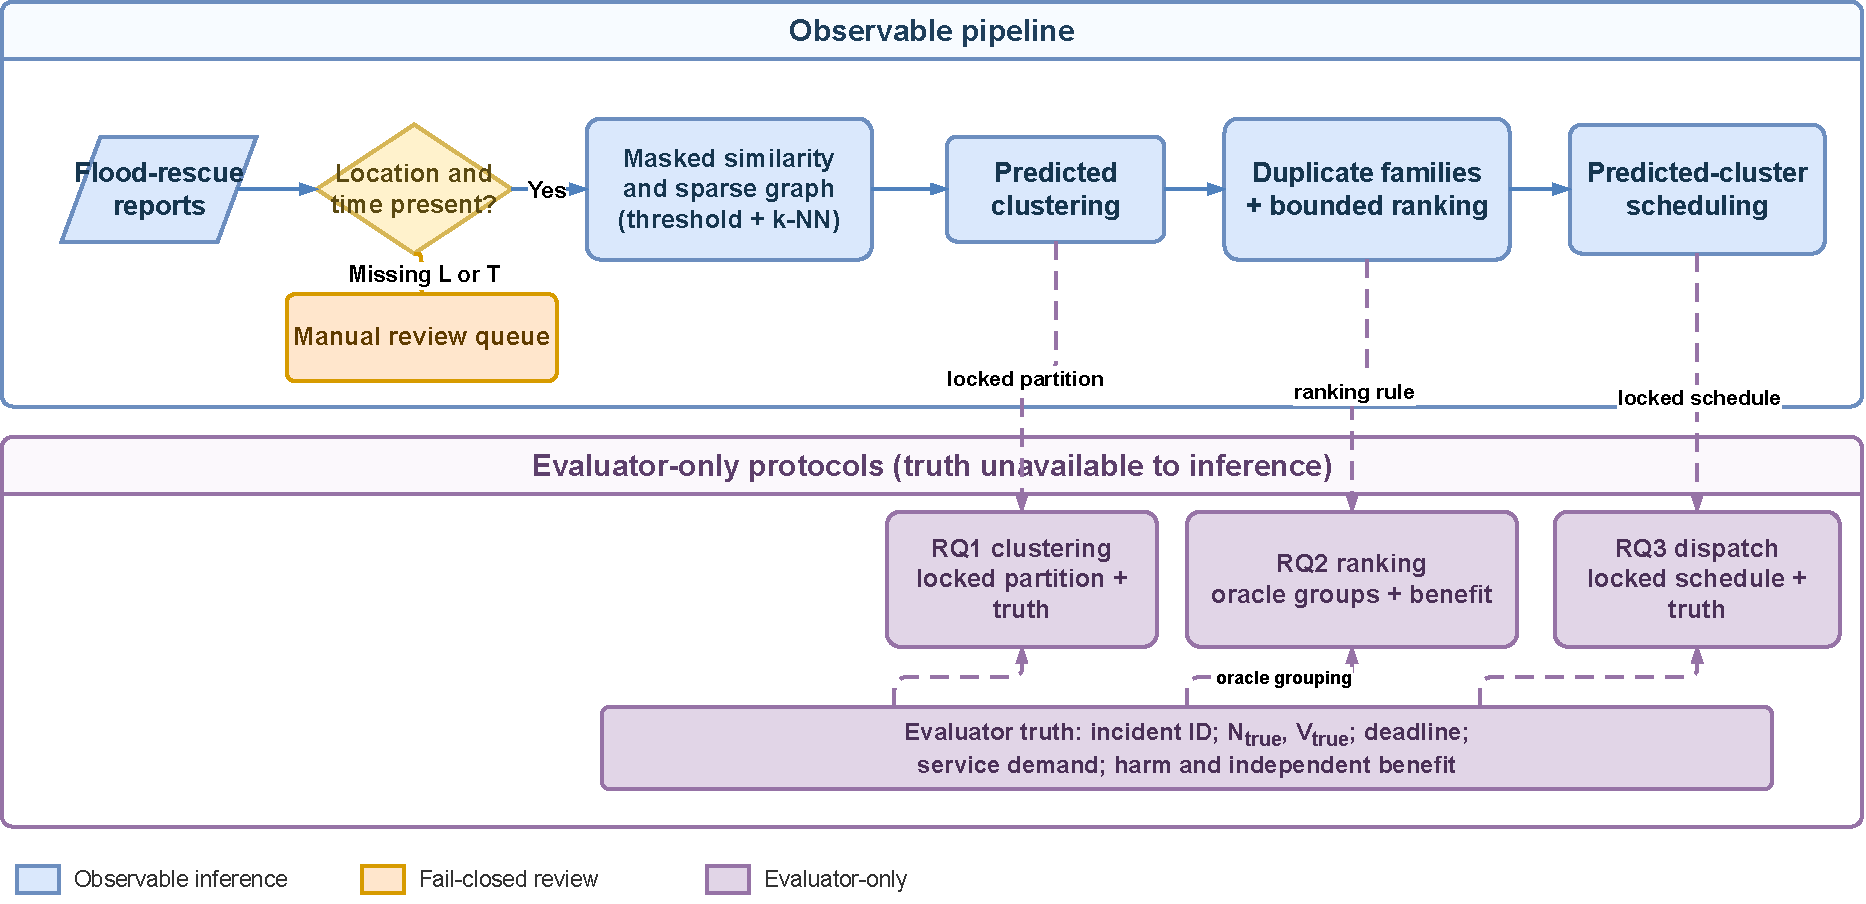
\includegraphics[width=\textwidth]{pipeline_v2.pdf}
\caption{Observable pipeline (solid), manual-review path (orange), and
evaluator-only truth join (dashed). The scheduler receives predicted clusters,
never incident truth.}
\label{fig:pipeline}
\end{figure}

Algorithm~\ref{alg:pipeline} restates this diagram as pseudocode: admission
gating and manual-review routing (Section~2.1), similarity-graph construction
and clustering (Section~2.2), duplicate-aware priority scoring
(Section~2.3, detailed as a subroutine in Algorithm~\ref{alg:priority}), and
the scheduler and evaluator-only truth join. Line numbers below correspond to
the equations introduced in the remainder of this section.

\begin{algorithm}[t]
\caption{Fail-closed observable report pipeline (Fig.~\ref{fig:pipeline})}
\label{alg:pipeline}
\begin{algorithmic}[1]
\Require Reports $R=\{r_i\}$; kernel scales $\sigma,\tau_t,\tau_F,\tau_E$;
weights $\beta,\gamma$ (and $\alpha$ for the additive composition); quantile
$q$; neighbour cap $k$; Louvain/Leiden resolution $\rho$; composition
$m\in\{\text{product},\text{additive}\}$
\Ensure Dispatch schedule $S$; the algorithm below never reads incident
identity, benefit, deadline, or harm labels
\State $R_{\rm obs}\gets\emptyset$; $R_{\rm review}\gets\emptyset$
\For{each report $r_i\in R$}
    \State $a_i\gets\mathbf{1}\{L_i,T_i\text{ observed}\}$ \Comment{Section~2.1}
    \If{$a_i=0$}
        \State $R_{\rm review}\gets R_{\rm review}\cup\{r_i\}$
        \Comment{orange manual-review path}
    \Else
        \State $Q_i\gets\operatorname{sigmoid}\bigl(b_0+b_1\mathbf{1}\{\text{image}_i\}
        +b_2\log(1+n_i^{\rm corrob})\bigr)$
        \State $R_{\rm obs}\gets R_{\rm obs}\cup\{r_i\}$
    \EndIf
\EndFor
\State $E\gets\emptyset$ \Comment{candidate edge set, Section~2.2}
\For{each $r_i\in R_{\rm obs}$}
    \State $K_i\gets$ the $\max(64,4k)$ nearest spatial neighbours of $r_i$ in
    $R_{\rm obs}$ (all boundary-distance ties included)
    \For{each $r_j\in K_i$}
        \State Compute $G_{ij}$, $T_{ij}$, and missingness-aware $C_{ij}$
        \If{$m=\text{product}$}
            \State $w_{ij}\gets a_ia_j\,G_{ij}(\beta T_{ij}+\gamma C_{ij})$
        \Else
            \State $w_{ij}\gets a_ia_j(\alpha G_{ij}+\beta T_{ij}+\gamma C_{ij})$
        \EndIf
        \State $E\gets E\cup\{(i,j,w_{ij})\}$
    \EndFor
\EndFor
\State $\theta\gets q$-quantile of the nonzero weights $\{w_{ij}:(i,j,w_{ij})\in E\}$
\State $E\gets\{(i,j,w_{ij})\in E:w_{ij}>\theta\}\ \cup\
\text{(endpoint-wise top-}k\text{ edges)}$
\State $\mathcal{G}\gets(R_{\rm obs},E)$
\State $\mathcal{C}\gets$ Louvain$/$Leiden$(\mathcal{G},\rho)$
\Comment{predicted clusters, never incident truth}
\State $\mathcal{F}\gets$ ExactFingerprintGroups$(R_{\rm obs})\ \cup\
$ NearDuplicateComponents$(R_{\rm obs})$ \Comment{Section~2.3}
\For{each family $g\in\mathcal{F}$}
    \State $P_g\gets$ \Call{PriorityScore}{$g$} \Comment{Algorithm~\ref{alg:priority}}
\EndFor
\State $S\gets$ Scheduler$(\mathcal{C},\{P_g\}_{g\in\mathcal{F}})$
\Comment{scheduler sees predicted clusters and $P_g$ only}
\State \Return $S$
\Statex
\Statex \emph{Evaluator-only, offline (dashed path in
Fig.~\ref{fig:pipeline}; executed only after $S$ is fixed):}
\State Join $S$ and $R_{\rm review}$ with ground-truth incident identity,
benefit, deadline, and harm labels
\State Compute ARI, NDCG@5, and the dispatch harm/deadline outcomes
reported in Section~4
\end{algorithmic}
\end{algorithm}

\begin{algorithm}[t]
\caption{\textproc{PriorityScore}: duplicate-aware bounded priority (Eq.~\ref{eq:priority})}
\label{alg:priority}
\begin{algorithmic}[1]
\Function{PriorityScore}{family $g$}
    \State $\bar E\gets\dfrac{\sum_{i\in g}Q_iE_i}{\max(1,\sum_{i\in g}Q_i)}$
    \Comment{confidence-weighted mean urgency within $g$}
    \State $\bar F\gets\max_{i\in g}Q_iF_i$
    \State $\widetilde N_i\gets\min(N_i,N_{\rm ref})$ for each $i\in g$
    \State $\bar N\gets\min\!\Bigl(1,\dfrac{\log\bigl(1+\max_{i\in g}Q_i\widetilde N_i\bigr)}
    {\log(1+N_{\rm ref})}\Bigr)$
    \State $\widetilde V_i\gets\min(V_i,V_{\rm cap})$ for each $i\in g$
    \State $\bar V\gets\max_{i\in g}Q_i\widetilde V_i$
    \State $P_g\gets\bigl[1+(\mu-1)\tanh(\bar V/s)\bigr]
    \bigl(\omega_E\bar E+\omega_F\bar F+\omega_N\bar N\bigr)$
    \State \Return $P_g$
\EndFunction
\end{algorithmic}
\end{algorithm}

\emph{[Authors: Eq.~\ref{eq:priority} as typeset sums/maximizes $\bar E,\bar
F,\bar N,\bar V$ over ``$g$'' and ``$i\in g$'' together, which would make
these quantities identical for every family and unable to support the
per-family NDCG@5 ranking used in Section~4. Algorithm~\ref{alg:priority}
above assumes the intended reading is per-family (max/sum over $i\in g$ only,
for the fixed family $g$ passed to the function). Please confirm this
matches the ranking notebook, and correct Eq.~\ref{eq:priority}'s subscripts
if it does not.]}

\subsection{Report Attributes and Missingness}

Each report is represented by the compact tuple
\[
r_i=(L_i,T_i,F_i,E_i,N_i,V_i,Q_i),
\]
where $L_i$ is a GPS location and $T_i$ is the observable report timestamp
(``created\_at''). Flood evidence $F_i$ and urgency evidence $E_i$ are in
$[0,1]$; $N_i\in\mathbb{Z}_{\geq0}$ is the reported trapped-person count;
$V_i\geq0$ is a vulnerability-evidence value; and $Q_i\in[0,1]$ is a
provenance/confidence heuristic. $Q_i$ is not a calibrated probability of
truth. The implementation also carries observable support fields such as
image presence, source type, province, and missing-field flags; these support
$Q_i$ and duplicate fingerprints but are not additional latent labels.

The score $Q_i$ is computed from observable image presence and a capped count
$n_i^{\rm corrob}$ of nearby corroborating payloads using the proposed
heuristic
\[
\begin{aligned}
Q_i&=\operatorname{sigmoid}\!\left(b_0+b_1\mathbf{1}\{\text{image}_i\}
 +b_2\log(1+n_i^{\rm corrob})\right),\\[-1mm]
&(b_0,b_1,b_2)=(-.2,1.4,.9).
\end{aligned}
\]
Here $\operatorname{sigmoid}(x)=(1+e^{-x})^{-1}$. This is a pipeline rule,
not a calibrated truth model. No independent receipt timestamp or source
family is assumed.

Following the general missing-variable kernel problem~\cite{smola2005missing},
we use the following fail-closed construction. The admission indicator
$a_i=\mathbf{1}\{L_i,T_i\text{ are observed}\}$.
Thus $a_i a_j=0$ prevents an edge involving a report whose geographic or
temporal separation is undefined; such a report follows the manual-review
path. Missing $F_i$ or $E_i$ is not zero-imputed: let $I_F(i,j),I_E(i,j)$
indicate that both reports share the corresponding observation and let
$m_{ij}=I_F(i,j)+I_E(i,j)$; then
\[
C_{ij}=\frac{m_{ij}}{2}\exp\!\left[-I_F(i,j)\frac{|F_i-F_j|}{\tau_F}
-I_E(i,j)\frac{|E_i-E_j|}{\tau_E}\right],
\quad C_{ij}=0\ \text{if }m_{ij}=0.
\]
When $m_{ij}=2$, both contextual fields are used; when $m_{ij}=1$, the
maximum contextual similarity is discounted to $1/2$; and when $m_{ij}=0$,
no contextual agreement is inferred. In the current 80-run artifact, every
report has location, event time, flood, and urgency. Hence $a_i=1$ and
$m_{ij}=2$ throughout the evaluated data, reducing the expression to
\[
C_{ij}=\exp\!\left[-\frac{|F_i-F_j|}{\tau_F}
-\frac{|E_i-E_j|}{\tau_E}\right].
\]
The missingness extension is specified and unit-tested, but missingness
robustness is not claimed as an empirical result of this benchmark.
\subsection{Similarity Graph and Derived Bounds}

For Haversine distance $d_{ij}$ and time difference $\Delta t_{ij}$, define
the Gaussian affinity~\cite{ng2001spectral} and exponential temporal decay
~\cite{zhou2013triggering}:
\begin{align}
G_{ij}&=\exp[-d_{ij}^{2}/(2\sigma^2)],&
T_{ij}&=\exp[-\Delta t_{ij}/\tau_t],\nonumber\\
w^\times_{ij}&=a_i a_jG_{ij}(\beta T_{ij}+\gamma C_{ij}),&
w^+_{ij}&=a_i a_j(\alpha G_{ij}+\beta T_{ij}+\gamma C_{ij}).
\label{eq:similarities}
\end{align}
The exponential form is a precedent, not a claim that the complete
missingness-aware expression is copied from prior work~\cite{billot2008exponential}.
The product is a spatial gate motivated by spatial--range products such as
bilateral filtering~\cite{tomasi1998bilateral}; both compositions and all
weights here are defined by this paper.
All scales $\sigma,\tau_t,\tau_F,\tau_E$ are strictly positive and the
weights are nonnegative. The implementation first forms a common spatial
candidate pool of at most $\max(64,4k)$ neighbours per eligible report,
including all boundary-distance ties before canonical truncation. It computes
an empirical nonzero-weight quantile, retains strict above-threshold edges,
keeps the union of endpoint-wise top-$k$ edges, and applies Louvain. Product
and additive candidates have the same pool and grid, but each family is
selected independently; the estimand is therefore a pipeline comparison, not
an operator-only causal effect. Because product and additive pipelines are
calibrated on separate quantile grids, reflecting how each would be tuned
independently in practice, we treat this independently calibrated contrast
as the primary estimand for RQ1 throughout the paper: it answers whether a
practitioner who tunes each pipeline separately, as would occur in practice,
obtains a net benefit from product composition. Section~\ref{sec:results}
also reports a matched-density contrast, which equalizes retained-edge
fraction and mean degree across compositions, as a secondary robustness
diagnostic that isolates the composition operator from calibration choices.

\begin{theorem}[Product edge localization]
Let $B=\beta+\gamma>0$. If a product edge with threshold $0<\theta<B$ is
retained, then
$d_{ij}<\sigma\sqrt{2\log(B/\theta)}$. For $\theta\ge B$ the strict retained
set is empty; for $\theta\le0$ the threshold alone gives no finite cutoff.
\end{theorem}
\begin{proof}
Since $a_ia_j\le1$ and $T_{ij},C_{ij}\le1$,
$w^\times_{ij}\le B\exp[-d_{ij}^{2}/(2\sigma^2)]$. Combining
$\theta<w^\times_{ij}$ with positivity and taking logarithms gives the bound;
the endpoint cases follow from the same inequality.
\end{proof}
This is an edge statement. A component-diameter claim additionally needs a
bounded observed hop diameter; long transitive chains remain possible.

\begin{corollary}[Conditional component bound]
In the finite product region, a connected component with unweighted observed
hop diameter $h<\infty$ and geographic diameter $D$ satisfies
$D<hr_\theta^\times$, where
$r_\theta^\times=\sigma\sqrt{2\log(B/\theta)}$. A singleton has $h=D=0$.
\end{corollary}
The result follows from the triangle inequality along a path of at most $h$
retained edges. It is a conditional post-hoc component bound, not an ex-ante
compactness guarantee: the pipeline does not control $h$.

For the additive form, assume $\alpha>0$. If
$B<\theta<B+\alpha$, every retained edge satisfies
\[
d_{ij}<r_\theta^+
=\sigma\sqrt{2\log\!\left(\frac{\alpha}{\theta-B}\right)}.
\]
If $\theta\ge B+\alpha$, the strict retained set is empty; if
$\theta\le B$, no non-trivial threshold-induced geographic cutoff exists in
general. Indeed, retention gives
$\theta<\alpha G_{ij}+\beta T_{ij}+\gamma C_{ij}\le\alpha G_{ij}+B$.
Thus product composition has a finite geographic edge bound throughout its
nonempty positive-threshold domain, whereas additive composition has such a
bound only above the maximum non-geographic contribution. Neither statement
alone implies better empirical clustering.

\subsection{Duplicate-Aware Bounded Ranking}

Exact duplicate payloads share a canonical fingerprint. Near duplicates are
joined by deterministic connected components under the observable envelope;
this transitive rule is not complete linkage. Let $g$ index the resulting
evidence families. The revised estimator uses confidence-gated family maxima
and avoids treating overlapping reports as disjoint people. Write
$\widetilde N_i=\min(N_i,N_{\rm ref})$ and
$\widetilde V_i=\min(V_i,V_{\rm cap})$ for the nonnegative clipped claims:
\begin{align}
\bar E&=\frac{\sum_g\max_{i\in g}Q_iE_i}
 {\max(1,\sum_g\max_{i\in g}Q_i)},&
\bar F&=\max_{g,i\in g}Q_iF_i,\nonumber\\
\bar N&=\min\!\left(1,\frac{\log(1+\max_{g,i\in g}Q_i\widetilde N_i)}
 {\log(1+N_{\rm ref})}\right),&
\bar V&=\max_{g,i\in g}Q_i\widetilde V_i,\nonumber\\
P&=\left[1+(\mu-1)\tanh(\bar V/s)\right]
 (\omega_E\bar E+\omega_F\bar F+\omega_N\bar N).
\label{eq:priority}
\end{align}
The candidate source snapshot associated with the RQ2/RQ3 artifacts specifies
$\omega=(.34,.33,.33)$, $\mu=2$, $s=10$, $N_{\rm ref}=500$, and
$V_{\rm cap}=50$. The formula is a proposed policy heuristic: maxima limit
duplicate multiplicity, the logarithm compresses heavy-tailed demand, clipping
bounds individual evidence, and the hyperbolic tangent saturates vulnerability
amplification. Reliability-aware truth discovery motivates using $Q_i$ but does
not derive these maxima~\cite{wang2012truth}. Transformation, normalization,
and weights require sensitivity and expert validation
~\cite{tate2012vulnerability,gralla2014review}; Section~\ref{sec:sensitivity}
reports a first such analysis. Comparators are a
multiplicity-sensitive legacy score, urgency-only, population-only, a simple
linear score, stable random, and---for dispatch---nearest-first.

\section{Experimental Design}

\paragraph{Data contract and splits.}
The artifact contains 80 independently seeded synthetic datasets
geographically anchored to the Copernicus EMSR848 Central Viet Nam flood
activation. Copernicus EMS, OpenStreetMap, and WorldPop provide geographic or
historical anchors; rescue incidents, reports, duplicates, coordinated
campaigns, vulnerability, and incident labels are synthetic. Every run has 16
latent incidents, 288--370 reports, exact and near duplicates, and three
coordinated nonincident campaigns of 20 reports each. Across all runs are
26,288 reports: 17,901 genuine, 3,587 duplicate, and 4,800 coordinated
nonincident reports. Runs 1--20 are reserved for development, runs 21--40 for
calibration, and runs 41--80 for held-out testing. All runs use one fixed
generator regime, so the experiment measures within-generator variation, not
mechanism-shift OOD transfer. Inference reads only
\texttt{algorithm\_input.json}; ground truth is opened after predictions for a
test run have been produced.

\paragraph{Selection and comparators.}
The current notebook evaluates complete small grids on the 20 calibration
runs and selects mean ARI, breaking ties by standard deviation and canonical
configuration JSON. Product and additive use fixed $\tau_F=.25$,
$\tau_E=.35$, and $\beta=\gamma=.5$. Selected product Louvain uses
$\sigma=700$ m, $\tau_t=60$ min, quantile $.90$, $k=8$, and resolution $1.2$.
Selected additive Louvain uses $\alpha=1$, $\sigma=700$ m, $\tau_t=60$ min,
quantile $.95$, $k=8$, and resolution $1.2$. Because selected quantiles
differ, this is an independently calibrated pipeline comparison, not a
matched-density operator comparison. Comparators are a convex similarity,
product Leiden, geo-time DBSCAN, DBSCAN/HDBSCAN on scaled observable features,
spatially constrained agglomerative clustering, and coordinate K-means. The
implemented geo-time DBSCAN lacks ST-DBSCAN's non-spatial criterion and is
named accordingly.

\paragraph{Endpoints and inference.}
ARI on incident-linked reports~\cite{hubert1985comparing} is the primary
endpoint; NMI, pairwise F1, geographic diameter, runtime, false destinations,
fake absorption, noise rejection, retained-edge fraction, and mean degree are
descriptive or operational diagnostics. The benchmark includes a matched-
density product--additive comparison. Seed-paired ARI differences use 10,000
bootstrap resamples, Wilcoxon signed-rank tests, and Holm correction. All Holm
corrections are applied within explicitly bounded hypothesis families, fixed
prior to inspecting held-out results: the RQ1 clustering family comprises the
product-vs-tuned-additive, product-vs-matched-density-additive, and
product-Leiden-vs-product-Louvain contrasts; the RQ2 ranking family comprises
the revised-vs-legacy, revised-vs-population-only, and revised-vs-random
NDCG@5 contrasts together with the coordinated-campaign drift contrast; and
the RQ3 dispatch family comprises the revised-vs-legacy, revised-vs-nearest,
and product-vs-matched-additive harm and deadline contrasts.
\emph{[Authors: confirm and, if needed, adjust the exact family membership
above against the analysis notebook before submission.]} The
priority stress tests and predicted-cluster dispatch evaluation use independent
benefit, deadline, service, access-delay, and harm outputs reported in Section~4;
no clustering metric is substituted for those outcomes.

\section{Results}
\label{sec:results}

In summary, across the 40 held-out test runs neither graph-clustering
composition shows a statistically robust advantage: additive Louvain attains
the highest mean ARI ($.9191$), but its margin over product variants does not
survive multiple-comparison correction under either calibration framing. For
priority ranking, the proposed duplicate-aware score removes duplicate
inflation but does not show a general alignment advantage over simpler
comparators, and is measurably more vulnerable than the legacy score to a
single realistic adversarial pattern---a coordinated high-confidence
reporting campaign. Downstream, these behaviors propagate into the dispatch
simulation: the revised policy shows no established improvement in harm or
deadline outcomes over the legacy score, and performs significantly worse
than a naive nearest-first baseline on both. The remainder of this section
presents the supporting statistical detail.

\begin{table}[t]
\centering\scriptsize
\caption{RQ1 benchmark-test summary over 40 runs. Intervals are bootstrap
95\% confidence intervals; diameter is descriptive.}
\label{tab:clustering-results}
\begin{tabular}{lccr}
\toprule
Method & ARI [95\% CI] & Pair F1 & Mean diam. (km)\\
\midrule
Additive Louvain & .9191 [.8995,.9381] & .9247 & .3477\\
Product Leiden & .9165 [.8979,.9351] & .9223 & .3547\\
Convex Louvain & .9135 [.8940,.9320] & .9195 & .3547\\
Product Louvain & .9072 [.8864,.9271] & .9138 & .3585\\
Matched-density Additive & .8973 [.8763,.9175] & .9046 & .3743\\
Coordinate K-means & .8176 [.7976,.8384] & .8292 & .2977\\
Spatial agglomerative & .6235 [.5964,.6494] & .6506 & 4.1648\\
HDBSCAN & .5205 [.4565,.5811] & .5787 & 1.2527\\
Geo-time DBSCAN & .4978 [.4589,.5366] & .5450 & .6244\\
DBSCAN, all features & .4741 [.4273,.5201] & .5488 & .9340\\
\bottomrule
\end{tabular}
\end{table}

Additive Louvain has the highest mean ARI. Product minus independently tuned
additive is $-0.01184$ with CI $[-0.02257,-0.00240]$, with 9 wins, 19 ties,
and 12 losses; raw $p=.0987$ and Holm $p=.2560$. Product minus matched-density
additive is $+0.00989$ with CI $[-0.00100,0.02082]$ and Holm $p=.2560$.
Product Leiden versus Product Louvain has Holm $p=.1120$. Thus neither
composition advantage is established. Product and matched-density additive
have nearly equal retained-edge fractions ($.03011$ and $.03021$) and mean
degrees (9.90 and 9.94), so the matched-density contrast is a useful diagnostic
but not a causal operator comparison.

The product pipeline has zero fake absorption and zero fake rejection but a
16.49\% false-destination rate; fake reports avoid genuine destinations while
still forming fake-only destinations. This is an adverse operational result,
not evidence of misinformation robustness.

\begin{figure}[t]
\centering
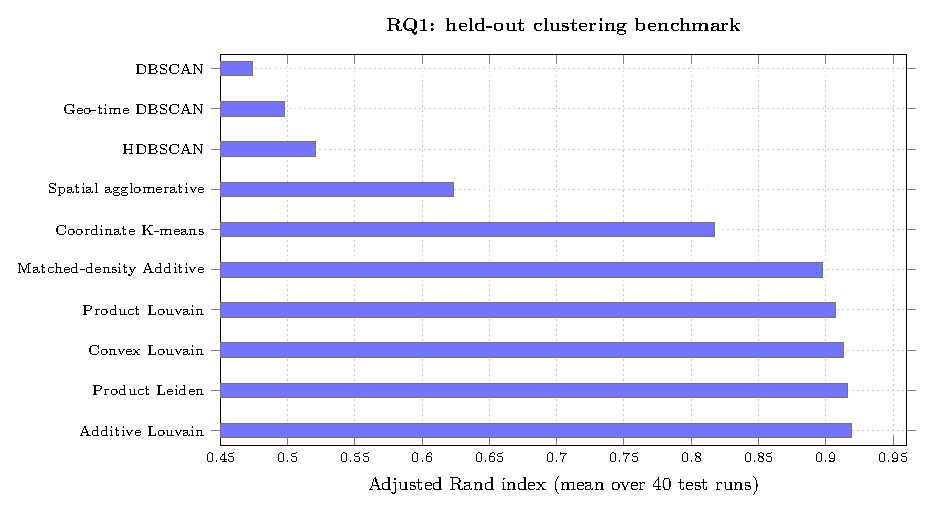
\includegraphics[width=\textwidth]{rq1_benchmark.pdf}
\caption{RQ1 held-out ARI means generated from the benchmark summary CSV.}
\label{fig:rq1-benchmark}
\end{figure}

\begin{table}[t]
\centering\scriptsize
\caption{Headline RQ2/RQ3 results from the candidate-4.1 artifacts. Positive
paired effects favor the revised candidate; lower-is-better metrics use the
artifact's oriented sign convention.}
\label{tab:stress-results}
\begin{tabular}{llrr}
\toprule
Question & Contrast and metric & Effect & Holm $p$\\
\midrule
RQ2 & Revised NDCG@5 (absolute) & .6669 & --\\
    & Random NDCG@5 (absolute) & .6763 & --\\
    & Revised $-$ legacy NDCG@5 & +.0121 & .5882\\
    & Exact-duplicate priority drift & 0 & --\\
    & Coordinated-campaign drift & .1688 & --\\
RQ3 & Revised $-$ legacy, Product harm & $-14.34$ & .675\\
    & Revised $-$ legacy, Product deadline & +.0188 & .160\\
    & Revised $-$ nearest, Product harm & $-69.88$ & $1.8\times10^{-7}$\\
    & Revised $-$ nearest, Product deadline & $-.1771$ & $3.0\times10^{-15}$\\
    & Product $-$ matched Additive harm & $-18.34$ & .000151\\
\bottomrule
\end{tabular}
\end{table}

For RQ2, revised NDCG@5 is .6669 (CI [.6306,.7018]), Spearman is -.0304
(CI [-.1165,.0549]), and top-five overlap is .285 (CI [.2349,.3400]). The
revised score is above legacy on NDCG@5 by .0121, but the Holm-adjusted
contrast is not significant; it is below population-only (.6709) and random
(.6763). Exact duplication at 2$\times$, 5$\times$, and 10$\times$ produces
zero revised priority drift. A coordinated high-confidence campaign produces
drift .1688 and false-priority lift .8828; revised drift is worse than legacy
by $-.1379$ (Holm $p\approx9.1\times10^{-12}$). Boundedness therefore does
not guarantee ranking reliability.

\begin{figure}[t]
\centering
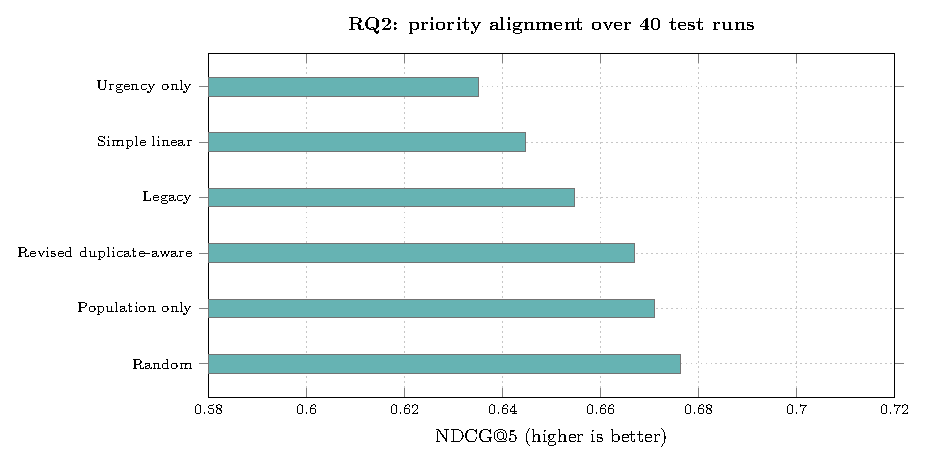
\includegraphics[width=\textwidth]{rq2_priority.pdf}
\caption{RQ2 priority-alignment comparison generated from the candidate-4.1
summary CSV.}
\label{fig:rq2-priority}
\end{figure}

For RQ3, revised versus legacy on the Product partition has harm effect
$-14.34$ (Holm $p=.675$) and deadline effect $+.0188$ (Holm $p=.160$), so no
general improvement is established. Revised is significantly worse than
nearest-first on both harm and deadline. Product is also worse than matched-
density Additive under the revised policy on harm, and worse than oracle on
the corresponding dispatch outcomes. Predicted split, merge, and fake-only
destinations therefore propagate into operational consequences.

\begin{figure}[t]
\centering
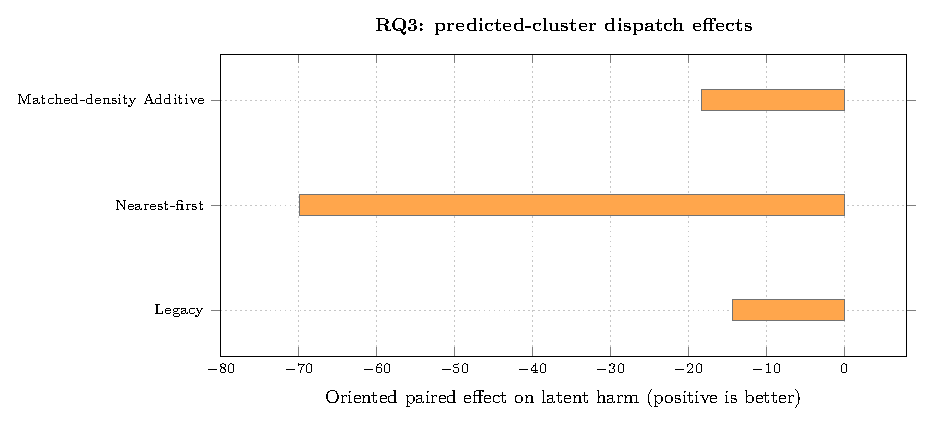
\includegraphics[width=\textwidth]{rq3_dispatch.pdf}
\caption{RQ3 Product-partition paired effects on latent harm generated from
the dispatch comparison CSV; positive values are improvement-oriented.}
\label{fig:rq3-dispatch}
\end{figure}

\subsection{Sensitivity of Heuristic Constants}
\label{sec:sensitivity}

To assess robustness to the fixed constants in $Q_i$ (Section~2.1) and $P$
(Eq.~\ref{eq:priority}), we perform a local one-at-a-time sensitivity
analysis: each constant is perturbed to $\pm20\%$ of its calibrated value
while holding all others fixed, and the headline held-out metric (mean ARI
for the clustering weights; NDCG@5 for the ranking constants) is recomputed
on the same 40 test runs. Table~\ref{tab:sensitivity} reports the resulting
metric range; a constant is considered stable if the metric varies by less
than $0.01$ across the perturbed range.

\begin{table}[t]
\centering\scriptsize
\caption{One-at-a-time sensitivity of headline metrics to fixed heuristic
constants ($\pm20\%$). \emph{[Authors: populate the Metric range column by
re-running the calibration notebook with each constant perturbed; do not
estimate these values.]}}
\label{tab:sensitivity}
\begin{tabular}{lccc}
\toprule
Constant & Calibrated value & Perturbed range & Metric range\\
\midrule
$b_0$ ($Q_i$ intercept) & $-0.20$ & $[-0.24,-0.16]$ & [FILL IN]\\
$b_1$ (image weight) & $1.40$ & $[1.12,1.68]$ & [FILL IN]\\
$b_2$ (corroboration weight) & $0.90$ & $[0.72,1.08]$ & [FILL IN]\\
$\omega$ ($\bar E,\bar F,\bar N$) & $(.34,.33,.33)$ & $\pm20\%$/component & [FILL IN]\\
$\mu$ (vulnerability amplification) & $2$ & $[1.6,2.4]$ & [FILL IN]\\
$s$ (vulnerability saturation) & $10$ & $[8,12]$ & [FILL IN]\\
$N_{\rm ref}$ & $500$ & $[400,600]$ & [FILL IN]\\
$V_{\rm cap}$ & $50$ & $[40,60]$ & [FILL IN]\\
\bottomrule
\end{tabular}
\end{table}

\section{Discussion and Threats to Validity}

The results separate mathematical safeguards from empirical utility. Product
gating supplies a finite edge bound in its positive-threshold domain, but the
independently tuned product pipeline does not outperform additive clustering.
The matched-density point estimate reverses the direction, yet its adjusted
test remains inconclusive. The graph theorem is therefore a localization
property, not evidence of a preferred composition.

The revised score removes exact-duplicate inflation and limits multiplicity,
but it does not show a general alignment advantage. Its coordinated-campaign
failure is especially important: an adversary can create a high-confidence
pattern that remains numerically bounded while still perturbing the ranking.
Dispatch results confirm that a bounded score cannot substitute for a
validated operational objective; clustering errors and fake-only destinations
are transmitted to scheduling.

All reports, incidents, relevance signals, and dispatch outcomes are
synthetic. RQ1 varies seeds within generator 3.0.0, while RQ2/RQ3 use a
separate candidate-4.1 bundle; neither tests mechanism-shift OOD transfer or
field performance. RQ1 does not provide an empirical missingness test because
all evaluated reports contain the four core attributes. No expert panel
validated the priority weights, caps, or utility. The study also does not
measure extraction accuracy, device latency, memory, energy, provenance
authenticity, or real-world harm. These limitations preclude policy or
deployment claims.

\section{Artifact and Conclusion}

The accompanying artifact contains the 80-run dataset, benchmark notebooks,
calibration grid, selected configurations, per-run test results, paired
comparisons, and the deterministic figure-generation script. The publication
figures are generated from the result CSVs; the original artifact PNGs remain
available for audit. Every reported number is generated from an accepted CSV
row and its documented generator and configuration metadata.

\paragraph{Data and Code Availability.}
The 80-run synthetic dataset, calibration grids, selected configurations,
benchmark notebooks, per-run results, and the deterministic
figure-generation scripts described above are available at
\url{[REPOSITORY URL]} under \texttt{[LICENSE]}. Reviewers may request
access to the artifact bundle prior to publication by contacting the
corresponding author. \emph{[Authors: replace with the actual repository
URL and license before submission.]}

In conclusion, the study establishes conditional graph bounds and documents
competitive within-generator clustering, exact-duplicate invariance, and
important negative results for ranking and dispatch. It does not establish
ranking alignment, dispatch benefit, misinformation robustness, policy
validity, or deployment readiness. The contribution is an auditable
stress-test boundary around those claims, not a validated rescue policy.

\bibliographystyle{splncs04}
\bibliography{references}

\end{document}
